\documentclass{article}

\usepackage[eandd,nonanonymous]{neurips_2026}

\usepackage{iftex}
\ifPDFTeX
\usepackage[utf8]{inputenc}
\fi
\usepackage[T1]{fontenc}
\usepackage{hyperref}
\usepackage{url}
\usepackage{booktabs}
\usepackage{amsfonts}
\usepackage{amsmath}
\usepackage{amssymb}
\usepackage{microtype}
\usepackage{xcolor}
\usepackage{graphicx}
\usepackage{enumitem}
\usepackage{multirow}
\usepackage{array}

\newcolumntype{L}[1]{>{\raggedright\arraybackslash}p{#1}}
\newcolumntype{C}[1]{>{\centering\arraybackslash}p{#1}}
\newcommand{\figtitle}[1]{\textbf{\footnotesize #1}}
\newcommand{\statusfrozen}{\textsc{Frozen}}
\newcommand{\statuspartial}{\textsc{Pre-formal}}
\newcommand{\statuspending}{\textsc{Pending}}
\newcommand{\barwithvalue}[2]{\raisebox{0.2ex}{\color{gray!35}\rule{#1}{1.15ex}}\,#2}

\title{DisasterAgentBench: An Evaluation Benchmark for Retrieval-Grounded Disaster Assessment with Drone-in-the-Loop Reinspection}

\author{%
  Haifeng Wang \\
  State Key Laboratory of Information Engineering in Surveying, Mapping and Remote Sensing \\
  Wuhan University \\
  Wuhan 430079, China \\
  \texttt{wanghaifeng68@whu.edu.cn} \\
  \And
  Wei He\thanks{Corresponding author.} \\
  State Key Laboratory of Information Engineering in Surveying, Mapping and Remote Sensing \\
  Wuhan University \\
  Wuhan 430079, China \\
  \texttt{weihe1990@whu.edu.cn} \\
}

\newcommand{\datasetfiles}{10{,}754}
\newcommand{\datasetevents}{298}
\newcommand{\datasethazards}{20}
\newcommand{\datasetgeojson}{563}
\newcommand{\datasetlabels}{258}
\newcommand{\datasetsarfiles}{10{,}184}

\begin{document}

\maketitle

\begin{abstract}
Existing agent benchmarks only weakly capture disaster assessment as a retrieval-grounded, map-grounded, and review-sensitive evaluation setting: a system must retrieve the correct event from a heterogeneous geospatial archive, ground its actions in the correct map source, localize evidence, decide whether drone reinspection is warranted, synthesize severity, and produce an auditable report. We present \textbf{DisasterAgentBench}, a benchmark and evaluation protocol for this workload, built from a disaster bundle containing \datasetfiles{} imagery layers, \datasetevents{} events, \datasethazards{} hazard categories, \datasetgeojson{} GeoJSON overlays, and \datasetlabels{} label files. The benchmark defines six task families, structured task records, explicit tool budgets, deterministic grading rules, a gold-removed hidden-test package, and review-aware metrics. We also provide \textbf{DisasterAgent}, a traceable reference baseline that makes the benchmark executable end to end. Evaluation on a 262-task hidden-test package shows a consistent diagnostic pattern: tool-equipped systems can saturate retrieval, grounding, and localization, while assessment synthesis, calibration, and report grounding remain difficult. The resulting comparison indicates that correct geospatial interaction does not by itself guarantee correct disaster judgment, and that the benchmark remains sensitive to downstream assessment quality even when upstream tool use is nearly saturated. The contribution is therefore a reproducible benchmark and evaluation protocol that separates geospatial tool access from disaster judgment quality.
\end{abstract}

\section{Introduction}

Disaster assessment is neither a single-step perception task nor a generic tool-use task. A capable agent must retrieve the correct event from a large heterogeneous geospatial archive, ground decisions on the correct map source, localize affected regions, determine whether uncertain evidence warrants UAV reinspection, and produce an auditable report with calibrated uncertainty. Errors in any early stage can invalidate the full decision chain, while correct upstream interaction still may not imply a correct downstream assessment. We therefore study disaster assessment as a benchmark problem involving retrieval-grounded, map-grounded, drone-in-the-loop agent behavior.

Existing benchmarks evaluate broad reasoning, web interaction, software repair, or app-centric workflows, and they have substantially advanced the study of tool-using language agents \citep{liu2024agentbench, mialon2024gaia, deng2023mind2web, zhou2023webarena, xie2024osworld, jimenez2024swe_bench, yao2024tau_bench, trivedi2024appworld}. However, they do not directly capture the coupled geospatial decision process required in disaster assessment: event retrieval from heterogeneous archives, map-source disambiguation, region-of-interest grounding, follow-up reinspection planning, and review-aware reporting. Conversely, traditional remote-sensing pipelines often assume fixed datasets, fixed models, or fixed interfaces, and therefore do not test whether an agent can manage the full decision loop.

Disaster assessment is a distinct agent problem for three reasons. First, correctness is event-conditioned: retrieving the wrong event or layer is a hard failure even if downstream reasoning is internally consistent. Second, evidence acquisition is adaptive rather than static: when map-side evidence is insufficient, the agent must decide whether and how to trigger UAV reinspection. Third, the setting is safety-sensitive: outputs should be uncertainty-aware, reviewable, and compatible with human override rather than optimized purely for autonomous completion.

To study this setting, we introduce \textbf{DisasterAgentBench}, a benchmark and evaluation protocol built from a curated disaster bundle spanning \datasetfiles{} imagery layers, \datasetevents{} events, \datasethazards{} hazard categories, \datasetgeojson{} GeoJSON overlays, and \datasetlabels{} label files. DisasterAgentBench defines six task families---event retrieval, map grounding, damage localization, drone reinspection, assessment synthesis, and report generation---under explicit tool budgets, structured task records, deterministic grading rules, hidden-test packaging, and held-out transfer hooks. The main contribution is the benchmark itself: a reproducible evaluation setting for a class of agent workload that existing benchmarks only weakly cover.

To make this evaluation setting executable end to end, the benchmark includes a reference implementation, a UAV reinspection environment, and evidence-trace interfaces that expose intermediate state for scoring and audit. \textbf{DisasterAgent} instantiates the reference baseline within this substrate, coupling archive retrieval, map interaction, tiled localization, UAV mission planning, assessment synthesis, and report generation under an explicit workflow trace. These components are included because they make the benchmark runnable, auditable, and diagnostically useful, not because the paper's primary claim depends on any one system component in isolation. More broadly, the benchmark turns post-disaster UAV reinspection into a shared evaluation substrate across multiple hazard and event scenarios, reducing the fragmentation that has made UAV-agent assessment difficult to compare across narrowly scoped setups.

The formal evaluation also motivates a benchmark-first reading rather than a simple architecture-ranking story. Tool-equipped systems saturate retrieval, grounding, and localization in the hidden-test run, but they differ sharply in drone execution, assessment synthesis, report grounding, calibration, latency, and traceability. In the present comparison, the completed systems occupy different operating points under the shared task definition and execution budget. DisasterAgentBench is useful precisely because it makes these tradeoffs measurable.

The paper is therefore organized around three benchmark design dimensions rather than around system-centric claims. First, the benchmark must capture event-grounded retrieval and map-grounded execution under realistic archive ambiguity. Second, it must expose long-horizon coordination demands rather than collapsing into one-shot perception or navigation. Third, it must evaluate safety-relevant assessment behavior, including reinspection decisions, uncertainty, and report grounding. The reference baseline and oracle controls are used only to operationalize these dimensions and to reveal which parts of the workflow are easy, which are brittle, and which remain the dominant bottlenecks under formal evaluation.

Our primary contribution is therefore not an application system, but an evaluation setting for a previously under-specified class of agent workloads. By turning disaster assessment into a benchmark with explicit task structure, evaluation protocol, execution constraints, and review-aware metrics, we aim to make this problem measurable, reproducible, and comparable across agent architectures. The central empirical question is correspondingly benchmark-centric: once systems can retrieve the right event and operate the right map tools, does correct geospatial interaction actually translate into correct disaster judgment?

\paragraph{Contributions.}
We make three contributions:
\begin{enumerate}[leftmargin=1.2em]
    \item We introduce \textbf{DisasterAgentBench}, an evaluation benchmark for retrieval-grounded, map-grounded, drone-in-the-loop disaster assessment, with six task families, structured task records, explicit tool budgets, deterministic grading rules, and hidden-test packaging.
    \item We provide the executable evaluation substrate for this benchmark, including \textbf{DisasterAgent} as a traceable reference baseline and a post-disaster UAV reinspection environment that makes reinspection tasks runnable, auditable, and comparable across hazard scenarios.
    \item We present a reproducible evaluation protocol, hidden-test result, validation checks, and oracle controls showing that correct archive and map interaction can saturate while assessment synthesis, calibration, and report grounding remain the dominant bottlenecks.
\end{enumerate}

\section{Related Work}

Our work sits at the intersection of language-agent architectures, realistic tool-use benchmarks, and geospatial disaster analysis. Surveys and architectural frameworks such as CoALA and recent LLM-agent surveys emphasize that strong agents require memory, planning, tool use, and environment grounding rather than prompt-only reasoning \citep{wang2024survey_llm_autonomous_agents, xi2025rise_potential_llm_agents, sumers2024coala}. Multi-agent frameworks such as AutoGen and Magentic-One further motivate explicit role decomposition and managed handoffs when tasks mix retrieval, execution, and synthesis \citep{wu2023autogen, fourney2024magentic_one}.

The closest prior evaluations come from realistic agent benchmarks. AgentBench and GAIA test broad reasoning and tool use \citep{liu2024agentbench, mialon2024gaia}. Mind2Web, WebArena, WebLINX, VisualWebArena, WorkArena, and OSWorld study grounded interaction in browsers and computer environments \citep{deng2023mind2web, zhou2023webarena, lu2024weblinx, koh2024visualwebarena, drouin2024workarena, xie2024osworld}. SWE-bench, $\tau$-bench, and AppWorld evaluate software repair, tool-agent-user interaction, and app-centric workflows \citep{jimenez2024swe_bench, yao2024tau_bench, trivedi2024appworld}. These benchmarks are invaluable, but they do not directly capture the geospatial retrieval, map-source ambiguity, and audit-oriented reporting required in disaster assessment.

Our benchmark is also related to remote sensing and disaster mapping pipelines, but the problem formulation is different. Traditional pipelines typically assume a fixed dataset, a fixed model, or a fixed user interface. DisasterAgentBench instead asks whether a tool-using language agent can solve the full decision chain: retrieve the right event, activate the right map source, localize relevant evidence, synthesize a severity judgment, and expose that judgment in a reviewable report.

\section{Task Setting and Benchmark Construction}

\subsection{Problem Formulation}

We formalize end-to-end disaster assessment as follows. Let $x$ be a user request, $\mathcal{A}$ a geospatial archive of indexed assets, $\mathcal{T}$ the allowed tool set, and $\tau=(a_1,\ldots,a_T)$ an agent trajectory of tool calls and intermediate observations. The agent must predict a structured output
\[
y = (e, m, g, u, s, c, r),
\]
where $e$ is an event identifier, $m$ is a map source or region-of-interest grounding decision, $g$ is an optional geospatial output such as GeoJSON, $u$ is an optional drone reinspection plan, $s$ is a severity label, $c$ is a calibrated confidence value, and $r$ is a structured report. Different benchmark tasks supervise different subsets of $y$, but all tasks preserve the same execution setting: archive retrieval, tool use, drone-aware follow-up planning, and evidence-grounded evaluation.

\subsection{Why Disaster Assessment Is a Distinct Agent Problem}

We define end-to-end disaster assessment as the following problem. Given a user request, an agent must (i) identify the relevant event and data assets, (ii) activate an appropriate map source or overlay, (iii) localize the target region or damaged objects, (iv) aggregate retrieved and detected evidence into an assessment, and (v) produce a structured report with explicit confidence. This workflow differs from standard web navigation because the target state is not merely an interaction trace; it is a grounded geospatial assessment whose correctness depends on retrieval, localization, synthesis, and auditability.

\subsection{Source Bundle}

Our benchmark is built from a local disaster bundle containing indexed geospatial layers and event metadata. Corpus-scale quantities are summarized in Appendix Table~\ref{tab:corpus-stats}, while split and hidden-test composition are reported separately in Appendix~\ref{sec:split-manifest-summary}. At the corpus level, the bundle is large enough to introduce realistic retrieval ambiguity, event diversity, and heterogeneous asset types, while still allowing event-balanced task construction.

\paragraph{Archive structure.}
The indexed source bundle mixes event-centric disaster areas, label files, and extracted project metadata. At the top-group level, the bundle contains 10{,}490 \texttt{disaster\_area} files, 258 \texttt{labels} files, and a small number of project-level metadata files. Only 36 events expose both area and label artifacts, while 263 are area-only and 5 are label-only. In the raw archive, `disaster\_area' files are heavily skewed toward SAR-style records (\datasetsarfiles{} files under a single \texttt{sar\_data} event), which means that a benchmark built directly by file frequency would be severely imbalanced. DisasterAgentBench is therefore designed to be \emph{event-balanced} rather than file-balanced: the unit of sampling is the event-task pair, not the raw file.

\subsection{Task Record and Task Families}

Each benchmark item is represented as a structured task record with the fields summarized in the accompanying JSON schema: task identifier, split, task family, user request, allowed tools, tool budget, context, gold output, evaluation specification, and metadata. This design has two goals. First, it allows all baselines to be run under a uniform tool budget. Second, it makes grading deterministic for tasks whose success depends on multiple partial outputs.

We currently define six core task families:
\begin{enumerate}[leftmargin=1.2em]
    \item \textbf{Event retrieval}: identify the correct event and relevant assets from a natural-language request.
    \item \textbf{Map grounding}: switch to the correct tile source, overlay, or region of interest.
    \item \textbf{Damage localization}: generate geospatial outputs that localize affected areas or objects.
    \item \textbf{Drone reinspection}: choose and parameterize a follow-up UAV mission over uncertain or high-impact regions.
    \item \textbf{Assessment synthesis}: infer severity, impact summary, and confidence from retrieved and visual evidence.
    \item \textbf{Report generation}: produce a structured analyst-facing report grounded in evidence.
\end{enumerate}

Unlike generic tool-use benchmarks, drone tasks are explicitly stateful. A drone task record therefore specifies not only the target region but also a simulator start state, an admissible mission family, acceptable interrupt actions, and a success condition over route completion or ROI coverage. This lets the benchmark distinguish between merely mentioning a UAV and proposing an operationally plausible reinspection workflow.

\subsection{Annotation Protocol and Splits}

We use an event-centric annotation protocol. For each task, annotators first select the target event, then specify one or more valid user requests, the permissible tool set, the target region or map source, and the gold outputs needed for deterministic evaluation. Assessment and report tasks also require evidence keys that specify the minimum facts or artifacts a valid answer must reference. Drone reinspection tasks additionally annotate a valid mission family, a route or coverage target, and whether pause, resume, or return-home actions would be acceptable under operator intervention. This protocol prevents benchmark success from collapsing into template matching on report text.

To avoid leakage between train, development, and evaluation, we use event-level splits. We also include hazard-held-out, region-held-out, and time-held-out settings to probe transfer. The benchmark includes a public development set and a hidden test set, and the split manifest is distributed with the benchmark metadata.

\section{Reference Baseline: DisasterAgent}

\subsection{System Overview}

DisasterAgent is a retrieval-grounded multi-agent framework designed to convert a high-level disaster request into geospatially grounded evidence and a structured assessment. The system comprises:
\begin{itemize}[leftmargin=1.2em]
    \item a \textbf{Data Agent} for indexed archive retrieval,
    \item a \textbf{Map Agent} for map source switching and overlay publication,
    \item a \textbf{Model Agent} for tiled real-time or background localization,
    \item a \textbf{Drone Agent} for simulated aerial reinspection under mission and operator-control constraints,
    \item an \textbf{Assessment Agent} for evidence synthesis and severity estimation,
    \item a \textbf{Report Agent} for report rendering,
    \item and an \textbf{Orchestration Agent} that routes and traces the workflow.
\end{itemize}

\begin{figure}[t]
    \centering
    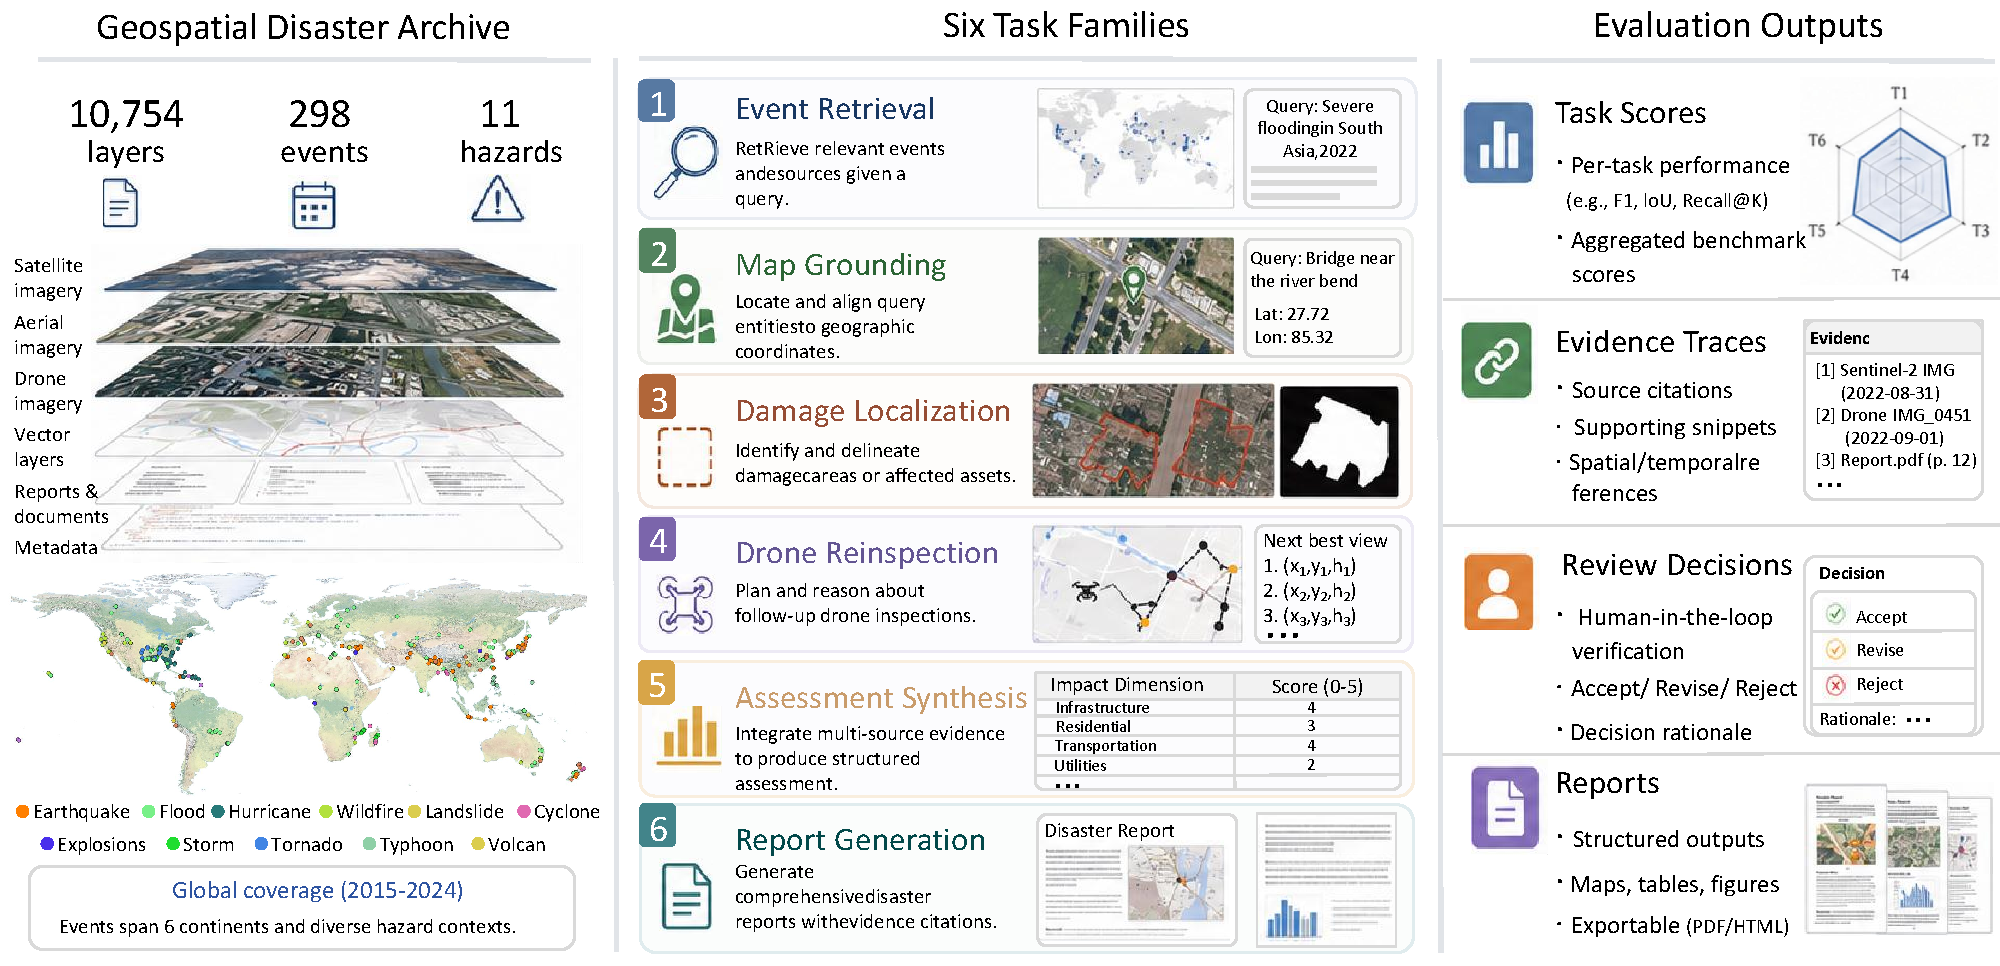
\includegraphics[width=\linewidth]{figs/001}
    \caption{DisasterAgentBench overview. The benchmark is built on a geospatial disaster archive with 10{,}754 files, 298 events, and 20 hazard types, and defines six task families evaluated through task scores, evidence traces, review decisions, and reports.}
    \label{fig:system}
\end{figure}

\subsection{Multi-Agent Task Orchestration}

DisasterAgent uses explicit workflow routing rather than an unconstrained planner. The orchestration layer selects among a small set of routes that cover retrieval, map preparation, localization, optional reinspection, assessment, and reporting. We represent a workflow as a directed acyclic graph
\[
W = (N, D),
\]
where nodes $N$ are agent-level stages and edges $D$ encode execution dependencies. A lightweight workflow bridge carries the upstream intent and routing decision across stages so that the benchmark can audit handoffs rather than only final outputs.

\subsection{Retrieval-Grounded Initialization}

The Data Agent searches a local indexed bundle of disaster assets and returns candidate map layers, overlays, or files associated with the requested hazard and event. Search operates over indexed metadata such as disaster type, event name, and file path, with query normalization for common hazard aliases. This stage matters because benchmark correctness is event-conditioned: a correct localization or report built on the wrong event is still a hard failure.

\subsection{Geospatial Tool Use}

After retrieval, the system prepares a displayable target, switches to a reachable tile source, publishes GeoJSON overlays, and passes the resulting context to the Model Agent. The Model Agent then performs tiled detection over either the present view or a larger background extent. For the benchmark, the key distinction is between \emph{where to look} and \emph{what to detect}.

\subsection{Drone Reinspection Execution Substrate}

To make drone tasks executable inside the benchmark, the Drone Agent runs in a simplified but stateful reinspection substrate for uncertain or high-impact regions. The simulator supports multiple mission families and explicit control interrupts such as pause, resume, stop, and return-home. Its role is benchmark-facing rather than aerodynamics-facing: it lets the evaluation score mission selection, region coverage, interruption handling, and operator escalation instead of treating UAV follow-up as a purely textual suggestion.

\subsection{Assessment Synthesis}

The Assessment Agent converts retrieved and visual evidence into a structured output with a severity label, confidence, metrics, recommendations, and an assessment overlay. Because this stage remains the least reliable part of the baseline, the benchmark pairs it with an explicit evidence-trace scaffold rather than treating the final assessment as an opaque score.

\subsection{Evidence-Trace Scaffold via HEG}

In the baseline, we use a lightweight \textbf{Hierarchical Evidence Graph (HEG)}-style scaffold to link retrieved assets, map views, detections, temporal comparisons, and review decisions. Its role here is pragmatic: it gives the benchmark an explicit evidence interface so that assessment and report tasks can be audited, graded, and ablated against a structured trace rather than a single opaque score. Let $G=(V,E)$ denote this evidence graph, where each node $v \in V$ has a type $t(v)$ and quality score $q(v)$, and each edge $(u,v)\in E$ has a relation type such as spatial overlap, temporal match, or support/conflict. We score severity class $k$ as
\[
S_k = \sum_{v \in V} \alpha_{t(v)} q(v)\phi_k(v) + \sum_{(u,v)\in E} \beta_{r(u,v)} \psi_k(u,v),
\]
where $\phi_k$ scores node-level support for class $k$ and $\psi_k$ scores pairwise consistency. The final severity prediction is $\hat{s}=\arg\max_k S_k$. We then compute a confidence score from graph agreement, conflict, and coverage:
\[
c = \sigma\!\left(\gamma_1 \operatorname{agreement}(G) - \gamma_2 \operatorname{conflict}(G) - \gamma_3 \operatorname{coverage\_gap}(G)\right).
\]
Within the benchmark, this scaffold provides severity estimation, calibrated confidence, and an explicit explanation path for analysts.

\subsection{Risk-Aware Review and Reporting}

Not every disaster task should be treated as fully autonomous. We therefore use a risk-aware review policy that routes uncertain or high-impact outputs to human review. A simple decision rule is
\[
\operatorname{review} = \mathbb{1}[c < \tau_c \ \lor\ (1-c)\cdot \operatorname{impact} > \tau_r],
\]
where $c$ is the calibrated confidence, $\operatorname{impact}$ is a task-level risk proxy, and $\tau_c,\tau_r$ are thresholds chosen on development data. The Report Agent renders the final structured output from the assessment trace, preserving severity, evidence, recommendations, and raw artifacts for audit.

\section{Evaluation Protocol}

\subsection{Benchmark Instantiation}

We instantiate DisasterAgentBench from the local indexed disaster bundle by sampling event-conditioned tasks rather than raw files. Each benchmark item specifies a user request, a task family, a split, an allowed tool set, and one or more gold targets. The source bundle exposes \datasetevents{} unique event names across \datasethazards{} hazard categories, but because several event names recur across different hazards, the split manifest is defined over 304 \emph{hazard-event} units rather than 298 bare event-name strings. Supervision is asymmetric: only 36 units provide paired \texttt{disaster\_area} and \texttt{labels} artifacts, whereas 263 are area-only and 5 are label-only. This asymmetry motivates family-specific task construction rather than a single uniform supervision recipe. The split manifest contains 212 train units, 46 development units, and 46 hidden-test units. The hidden-test package materializes these units into 262 gold-removed task records. That is, the hidden-test split is released as task instances with inputs and metadata but with gold outputs withheld for evaluation. Appendix Table~\ref{tab:family-eligibility} makes the counting policy explicit by separating families whose candidate pools are already derivable from the manifest from those that still depend on frozen severity or evidence annotations.

The split is broad enough to support nontrivial generalization claims even before the final task records are frozen. Training currently covers all 20 hazard categories represented in the bundle, while the public development and hidden-test manifests each cover 15 hazards. The largest hazard families are approximately stratified across splits: flooding contributes 45/10/10 train/dev/hidden-test units, Hurricane contributes 35/7/7, and Earthquake contributes 23/5/5. Split-level supervision composition is summarized in Appendix Table~\ref{tab:split-summary}; importantly, paired area+label units remain rare in every split, so evaluation should not assume dense supervision outside a small subset of events.

\subsection{Task Instantiation and Difficulty Control}

The benchmark is instantiated from \emph{hazard-event} units rather than raw files. Event-retrieval and map-grounding tasks require retrievable and displayable assets; localization tasks require geometry from \texttt{disaster\_area} or \texttt{labels}; drone tasks require an ROI plus an executable mission template; assessment and report tasks require severity targets and evidence keys. We use explicit \texttt{easy}/\texttt{medium}/\texttt{hard} buckets defined by retrieval ambiguity, map-source ambiguity, spatial scale, temporal complexity, and review requirement, so that the benchmark remains balanced across families and difficulty levels rather than being dominated by easy retrieval items.

\subsection{Evaluation Settings and Leakage Control}

We use event-level train/dev/test partitioning as the default split rule, so that all artifacts associated with the same disaster event remain in a single split. In practice, the split manifest uses hazard-stratified hazard-event units, deterministic hash ordering within each hazard, and minimum development/hidden-test allocations for hazards with at least four events. This is especially important because file-level splitting would be dominated by the \texttt{sar\_data} subtree, which contributes \datasetsarfiles{} files under a single event identifier and would otherwise swamp the benchmark. In addition to the default split, the benchmark exposes hazard-held-out, region-held-out, and time-held-out settings for transfer analysis. Hidden-test evaluation is distributed as task records without gold outputs. This protocol is intended to prevent leakage through repeated event identifiers, overlapping pre/post assets, or duplicated geospatial extents, while preserving event-balanced evaluation despite severe file-level skew.

We use four evaluation settings: \textbf{Event-IID} for the main table, plus \textbf{hazard-held-out}, \textbf{region-held-out}, and \textbf{time-held-out} for transfer. All prompts, routing rules, and review thresholds are tuned once on the public Event-IID development split and then frozen for all hidden-test and held-out evaluations.

\subsection{Comparison Systems}
\label{sec:comparison-systems}

Our target comparison set under matched tool budgets is:
\begin{enumerate}[leftmargin=1.2em]
    \item a direct LLM baseline without external tools,
    \item a single-agent ReAct-style tool user \citep{yao2023react},
    \item a retrieval-plus-detector pipeline without explicit orchestration,
    \item a single-agent system with the full tool set but no explicit workflow routing,
    \item an oracle-retrieval variant that receives the correct event context but still performs downstream map, detection, and assessment steps,
    \item the full DisasterAgent system,
    \item and a human-reference workflow on a stratified subset of tasks.
\end{enumerate}

This comparison set separates retrieval errors from downstream orchestration and assessment errors; the oracle-retrieval variant is particularly useful for measuring how much difficulty remains after event grounding is solved.
The hidden-test table in Section~\ref{sec:results} includes the full comparison set, but only the four tool-equipped systems have completed adjudicated runs under the frozen evaluation protocol; the direct-LLM, retrieval-plus-detector, and human-reference controls are therefore shown as intentionally unpopulated rows.

\subsection{Benchmark Validation Protocol}

Because DisasterAgentBench is positioned as an Evaluations \& Datasets contribution, benchmark validation must precede model interpretation. The validation suite reports coverage and diversity, agreement on a dual-annotated subset, oracle execution validity, human/reference solvability on a stratified subset, and ranking stability under resampling or repeated runs. Appendix~\ref{tab:benchmark-validation} records the validation snapshot. The human-annotation files now enter that snapshot directly: the 44-task \texttt{assessment\_synthesis} subset has overlapping A1/A2 labels for dual-annotator agreement, while the remaining families are covered by single-annotator checks against frozen references. The formal oracle rows, by contrast, come from hidden-test executions. Quantities that have not yet been populated under the boundary remain blank rather than being estimated from earlier traces.

\subsection{Metrics and Statistical Protocol}

We group metrics into four levels:
\begin{itemize}[leftmargin=1.2em]
    \item \textbf{Benchmark-quality metrics}: execution-validity rate, annotation agreement, human/reference success, and ranking stability.
    \item \textbf{Task metrics}: top-1 event accuracy, top-$k$ recall, grounding success, center distance, GeoJSON F1/IoU, mission validity, ROI coverage, intervention success, severity F1, and report grounding score.
    \item \textbf{System metrics}: end-to-end success, latency, tool calls, and runtime cost.
    \item \textbf{Risk metrics}: ECE, review rate, false-autonomy rate, and unnecessary-review rate.
\end{itemize}

For drone tasks, we separate \emph{mission validity} from \emph{geometric coverage}. If $P$ denotes the planned or executed flight path and $R$ denotes the target reinspection region, we score ROI coverage as
\[
\operatorname{coverage}(P,R) = \frac{\operatorname{area}(\operatorname{buffer}(P,\rho)\cap R)}{\operatorname{area}(R)},
\]
where $\rho$ is a fixed visibility radius derived from altitude and sensor assumptions. We report intervention compliance separately by checking whether the system preserves or correctly executes required pause, resume, stop, or return-home actions under the task specification.

\paragraph{Partial credit.}
Some tasks admit partial success. For example, a system may retrieve the correct event but fail to select the optimal map source, or it may localize the correct region while underestimating severity. The task schema therefore stores both a primary metric and optional thresholded grading rules such as center-distance thresholds, minimum IoU, or minimum ROI coverage.

\paragraph{Statistical protocol.}
All stochastic systems should be run with at least three seeds. Main tables should report means with 95\% bootstrap confidence intervals, and main pairwise claims should use paired bootstrap or approximate randomization on hidden-test predictions. Review and calibration thresholds must be fixed on development data before hidden-test evaluation.

\subsection{Implementation and Execution Protocol}

All baselines run against the same indexed archive, map interface, tiled model backend, and drone simulator. Every run logs the tool trace, intermediate artifacts, runtime, and final report. We also report \emph{infrastructure-induced failure} separately from reasoning failure so that backend outages are not misread as cognitive agent errors. Appendix~\ref{sec:execution-plan} converts this setup into a concrete freeze-run-score workflow, including which subsets populate each table, which variants require three seeds, and which artifacts must be saved for audit.

\section{Results}
\label{sec:results}

We report the hidden-test comparison on the 262-task Event-IID hidden-test package using the frozen evaluation configuration. Table~\ref{tab:main-results} summarizes the completed runs for the comparison systems and oracle controls under the shared benchmark setting. The single-agent and oracle baselines are averaged over three seeds, while the full-DisasterAgent row is populated from the execution budget used for the benchmark. Additional robustness, review, ablation, and trace-diagnostic panels remain in Appendix~\ref{sec:appendix-benchmark-diagnostics}.

Throughout this section, we distinguish \emph{execution success} from \emph{task success}. Execution success means that a run completes without infrastructure failure, policy interruption, or scorer-level invalidation; task success means that the task meets its declared primary metric threshold and therefore contributes positively to end-to-end benchmark success. This distinction matters because a system may execute the full workflow and still fail the benchmark on semantic assessment or report grounding.

\refstepcounter{table}\label{tab:main-results}
\begin{center}
    \scriptsize
    \setlength{\tabcolsep}{2.5pt}
    \textbf{Table~\thetable: Hidden-test comparison.} Columns report the family-level primary metrics together with end-to-end success, calibration, latency, and tool use on the 262-task hidden-test split under the frozen evaluation configuration. Single-agent and oracle baselines are means over three seeds; the full-DisasterAgent row is populated from the execution budget used for the benchmark. Empty cells denote comparison conditions that remain unpopulated under the frozen boundary.
    \vspace{0.35em}

    \begin{tabular}{lcccccccccc}
        \toprule
        System & Retr. & Ground. & Local. & Drone & Assess. & Report & E2E & ECE & Latency & Tools \\
        \midrule
        Single-agent ReAct & 1.000 & 1.000 & 1.000 & 0.000 & 0.500 & 0.278 & 0.588 & 0.285 & 0.106 & 5.511 \\
        Single-agent full tools & 1.000 & 1.000 & 1.000 & 1.000 & 0.500 & 0.278 & 0.748 & 0.199 & 0.115 & 5.000 \\
        Oracle grounding single-agent & 1.000 & 1.000 & 1.000 & 0.000 & 1.000 & 0.278 & 0.672 & 0.050 & 0.105 & 4.511 \\
        Oracle retrieval single-agent & 1.000 & 1.000 & 1.000 & 0.000 & 0.500 & 0.278 & 0.588 & 0.269 & 0.105 & 4.511 \\
        Oracle all gold & 1.000 & 1.000 & 1.000 & 1.000 & 1.000 & 1.000 & 1.000 & 0.010 & 0.000 & 0.000 \\
        Full DisasterAgent & 1.000 & 1.000 & 1.000 & 1.000 & 0.114 & 0.222 & 0.683 & 0.686 & 3.970 & 2.008 \\
        \bottomrule
    \end{tabular}
\end{center}

The main result is benchmark-centric. First, explicit access to the full geospatial tool chain is sufficient to saturate retrieval, grounding, and localization: every completed system reaches 1.000 on those upstream families. Second, the supporting oracle rows show that the remaining difficulty is structured rather than monolithic: improving access to correct event context can raise downstream performance, but does not by itself eliminate assessment, reporting, or execution bottlenecks. Third, the two baselines without a viable drone path collapse to 0 on the drone family and accumulate infrastructure-failure mass on those blocked trajectories, confirming that executable reinspection is a substantive part of the benchmark rather than a cosmetic tool hook.

Taken together, these results clarify what DisasterAgentBench measures. The benchmark is not limited by archive lookup or basic map interaction; instead, it remains sensitive to the harder problem of converting correct geospatial interaction into correct, calibrated, and analyst-ready disaster judgment. The non-oracle systems differ in end-to-end score, latency, calibration, and report grounding, but the more important observation is that upstream competence does not guarantee downstream assessment quality. In this sense, the comparison is useful because it separates \emph{tool access} from \emph{decision quality}, and also \emph{execution efficiency} from \emph{workflow governability}, under a shared task definition and matched execution constraints. Appendix Figure~\ref{fig:takeaway-profile} visualizes this upstream-versus-downstream gap directly.

\section{Limitations and Broader Impact}

The benchmark is derived from a locally curated disaster bundle and will likely inherit collection biases across hazard types, regions, and annotation styles. Some hazards may be overrepresented, while others may only appear in weakly labeled form. The UAV environment, while more realistic than a static waypoint player, is still not a full physical or regulatory simulator; it models operational decision variables such as mission mode, route, pause/resume, and return-home, but not full weather, battery chemistry, or communications failure. The DisasterAgent result should therefore be read as a reference point for the present implementation and evaluation budget, not as a ceiling on structured multi-agent orchestration. The present validation snapshot, while grounded in provided human annotations, still falls short of a fully adjudicated multi-family human study because only the assessment subset has dual annotation. Moreover, agent evaluation in disaster settings is safety-critical: overconfident outputs can mislead analysts, while underconfident systems may increase review burden and latency. We therefore recommend that all benchmark tasks preserve evidence traces, explicit uncertainty fields, and clear disclaimers against fully autonomous operational use.

\paragraph{Release scope.}
The benchmark distribution exposes the split-manifest metadata, task schema, frozen evaluation configuration, hidden-test package, scorer-facing task records, and aggregated run files needed to reproduce reported tables. The underlying local disaster bundle is not treated as an automatically redistributable corpus asset; where licenses or source restrictions prevent direct redistribution, the distribution boundary falls back to task-level metadata, frozen prompts and thresholds, and evaluator-side prediction and trace files.

\section{Conclusion}

Disaster assessment exposes a class of agent workload that benchmarks only weakly cover: event-grounded retrieval over large geospatial archives, map-source disambiguation, localized damage analysis, drone-assisted follow-up, and uncertainty-aware reporting. The main contribution of this paper is \textbf{DisasterAgentBench}, a benchmark and evaluation protocol for this setting. The benchmark is accompanied by an executable reference substrate, including a baseline implementation, a UAV environment, and evidence-trace interfaces that make reinspection-aware and review-aware evaluation operational rather than purely conceptual. By grounding this evaluation substrate in multi-hazard, multi-event disaster data, the benchmark provides a shared post-disaster UAV-agent setting in which mission selection, route execution, interruption handling, and evidence-grounded follow-up can be compared under one formal task definition. The benchmark now includes a 262-task gold-removed hidden-test package, a frozen evaluation configuration, and an initial hidden-test result. The main empirical takeaway is that correct geospatial interaction is not yet equivalent to correct disaster judgment, and that this gap remains measurable even when upstream retrieval and grounding are nearly saturated. By packaging task families, split design, grading rules, and a concrete freeze-run-score workflow, we aim to make this benchmark class reproducible, diagnosable, and comparable across agent architectures.

\bibliographystyle{plainnat}
\bibliography{agent_references}

\appendix

\section{Formal Evaluation Supplement}
\label{sec:appendix-benchmark-diagnostics}

This appendix contains supplementary formal-evaluation material that supports the main benchmark claim without consuming main-paper pages. It records frozen protocol components, supplementary evaluation slices, and diagnostic artifacts that complement the main hidden-test result.

\begin{table}[ht]
    \centering
    \caption{Corpus-scale benchmark statistics from the indexed disaster bundle. Split composition and hidden-test counts are reported separately from these source-bundle totals.}
    \label{tab:corpus-stats}
    \begin{tabular}{lr}
        \toprule
        Statistic & Value \\
        \midrule
        Imagery layers & \datasetfiles{} \\
        Hazard categories & \datasethazards{} \\
        Event identifiers & \datasetevents{} \\
        GeoJSON overlays & \datasetgeojson{} \\
        Label files & \datasetlabels{} \\
        Hazard-event split units & 304 \\
        Paired area+label events & 36 \\
        Area-only events & 263 \\
        Label-only events & 5 \\
        Task families & 6 \\
        \bottomrule
    \end{tabular}
\end{table}

\begin{table}[ht]
    \centering
    \small
\caption{Benchmark-validation snapshot. The human-annotation files support two distinct checks: dual-annotator agreement on the \texttt{assessment\_synthesis} subset, and broader single-annotator consistency checks against frozen references on the remaining families. Empty cells indicate validations reserved in the formal protocol but not yet populated by adjudicated runs.}
    \label{tab:benchmark-validation}
    \begin{tabular}{L{0.34\linewidth}L{0.22\linewidth}L{0.30\linewidth}}
        \toprule
        Validation quantity & Value & Notes \\
        \midrule
        Hidden-test task coverage & 262 tasks / 6 families & Event-IID hidden-test package \\
        Hazard coverage in split manifest & 15 hidden-test hazards & split-level statistic \\
        Human-label coverage & 306 provided labels / 262 task instances & assessment has dual annotation; the other families currently have single-annotator coverage \\
        Dual-annotated subset & 44 assessment tasks & provided A1/A2 labels with task-level overlap only on the assessment family \\
        Assessment agreement & 0.432 severity agreement & Cohen's $\kappa=0.210$ and evidence F1 1.000 on the dual-annotated assessment subset \\
        Oracle execution validity & oracle-all-gold E2E 1.000 & formal 3-seed oracle validation on all 262 tasks \\
        Single-annotator reference checks & 5 remaining families + assessment pass & broader family coverage uses one provided annotator checked against frozen references \\
        Ranking stability & 12 grouped systems / 66 pairwise tests & 3-seed aggregation over the main-table systems and six formal ablations \\
        \bottomrule
    \end{tabular}
\end{table}

\begin{figure}[ht]
    \centering
    \small
    \setlength{\tabcolsep}{6pt}
    \begin{tabular}{lll}
        \toprule
        System & Upstream execution profile & Downstream synthesis profile \\
        \midrule
        Single-agent ReAct & \barwithvalue{2.25cm}{0.750} & \barwithvalue{1.17cm}{0.389} \\
        Single-agent full tools & \barwithvalue{3.00cm}{1.000} & \barwithvalue{1.17cm}{0.389} \\
        Oracle retrieval single-agent & \barwithvalue{2.25cm}{0.750} & \barwithvalue{1.17cm}{0.389} \\
        Oracle grounding single-agent & \barwithvalue{2.25cm}{0.750} & \barwithvalue{1.92cm}{0.639} \\
        Oracle all gold & \barwithvalue{3.00cm}{1.000} & \barwithvalue{3.00cm}{1.000} \\
        Full DisasterAgent & \barwithvalue{3.00cm}{1.000} & \barwithvalue{0.50cm}{0.168} \\
        \bottomrule
    \end{tabular}
    \caption{Benchmark takeaway profile on the hidden test. The upstream score is the mean of retrieval, grounding, localization, and drone metrics; the downstream score is the mean of assessment and report metrics. The gap between the two columns visualizes the main claim of the benchmark: correct archive and map interaction do not imply correct synthesis or report grounding.}
    \label{fig:takeaway-profile}
\end{figure}

\begin{figure}[ht]
    \centering
    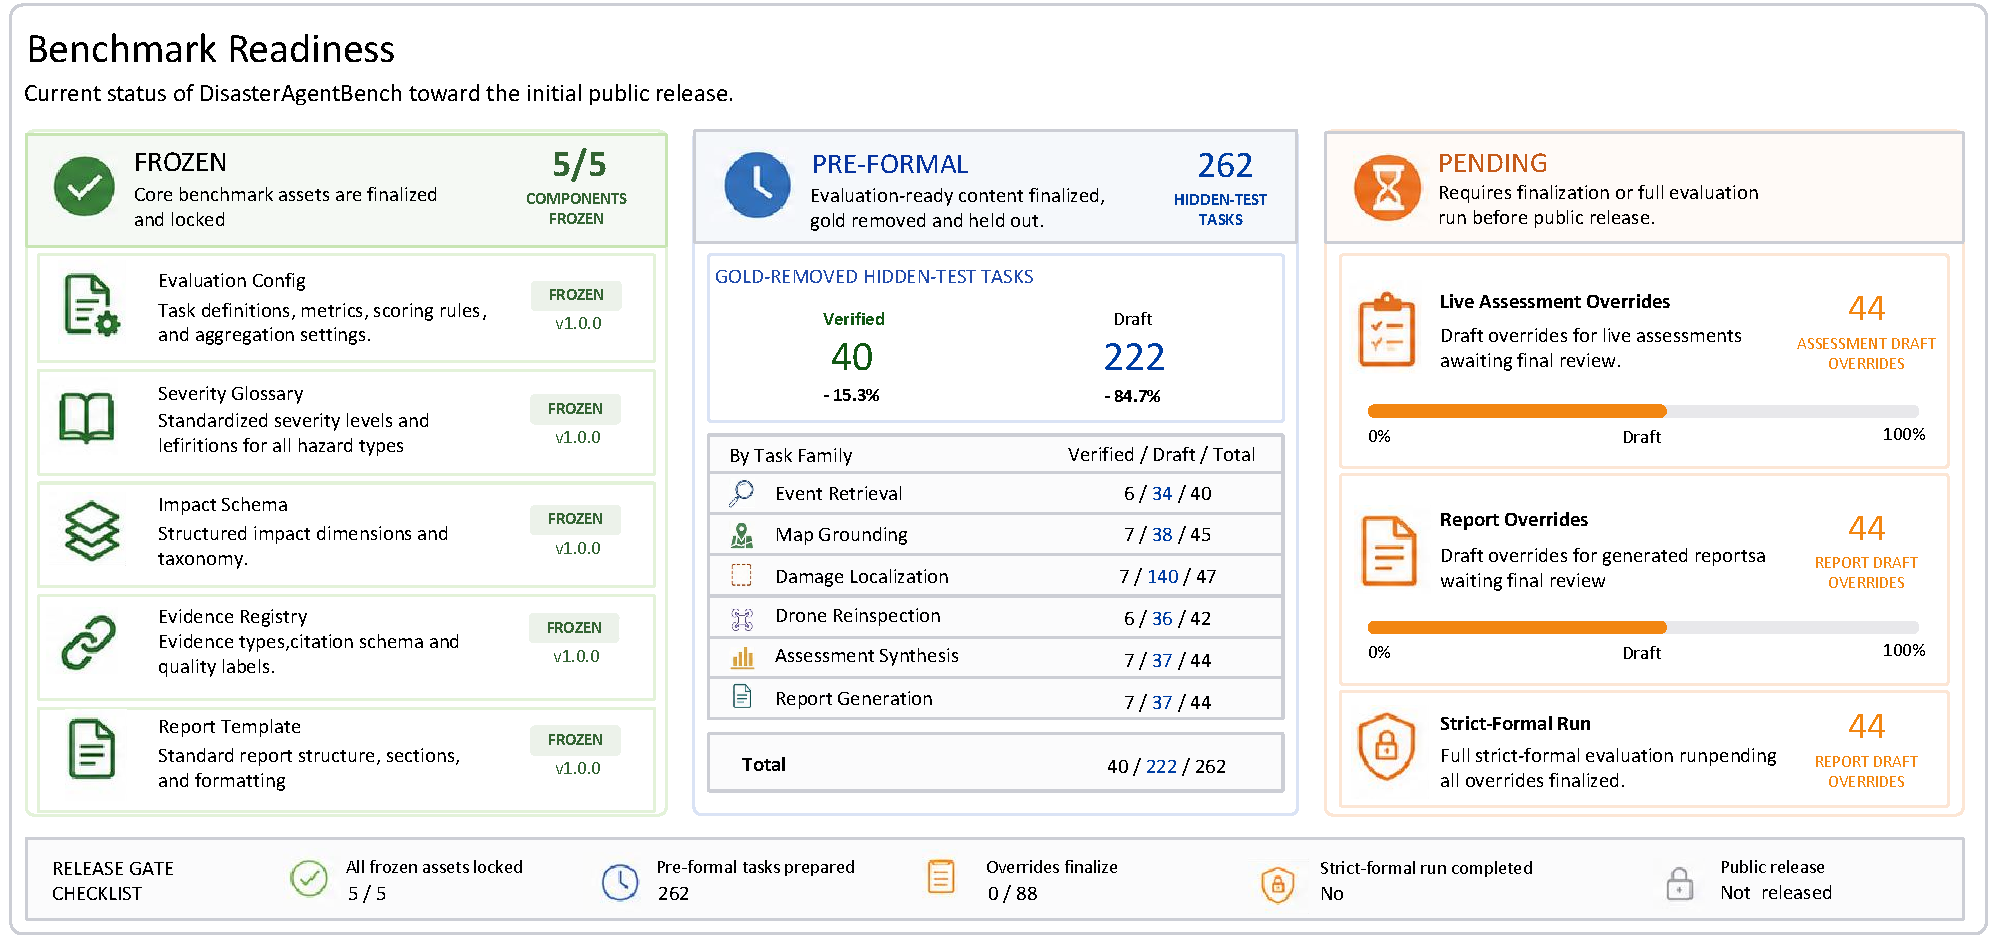
\includegraphics[width=\linewidth]{figs/002}
    \caption{Benchmark formalization ledger. The figure summarizes the frozen infrastructure, adjudication boundary, and evaluation state transitions that define the formal benchmark used for hidden-test scoring.}
    \label{fig:review-quality}
\end{figure}

\begin{figure}[ht]
    \centering
    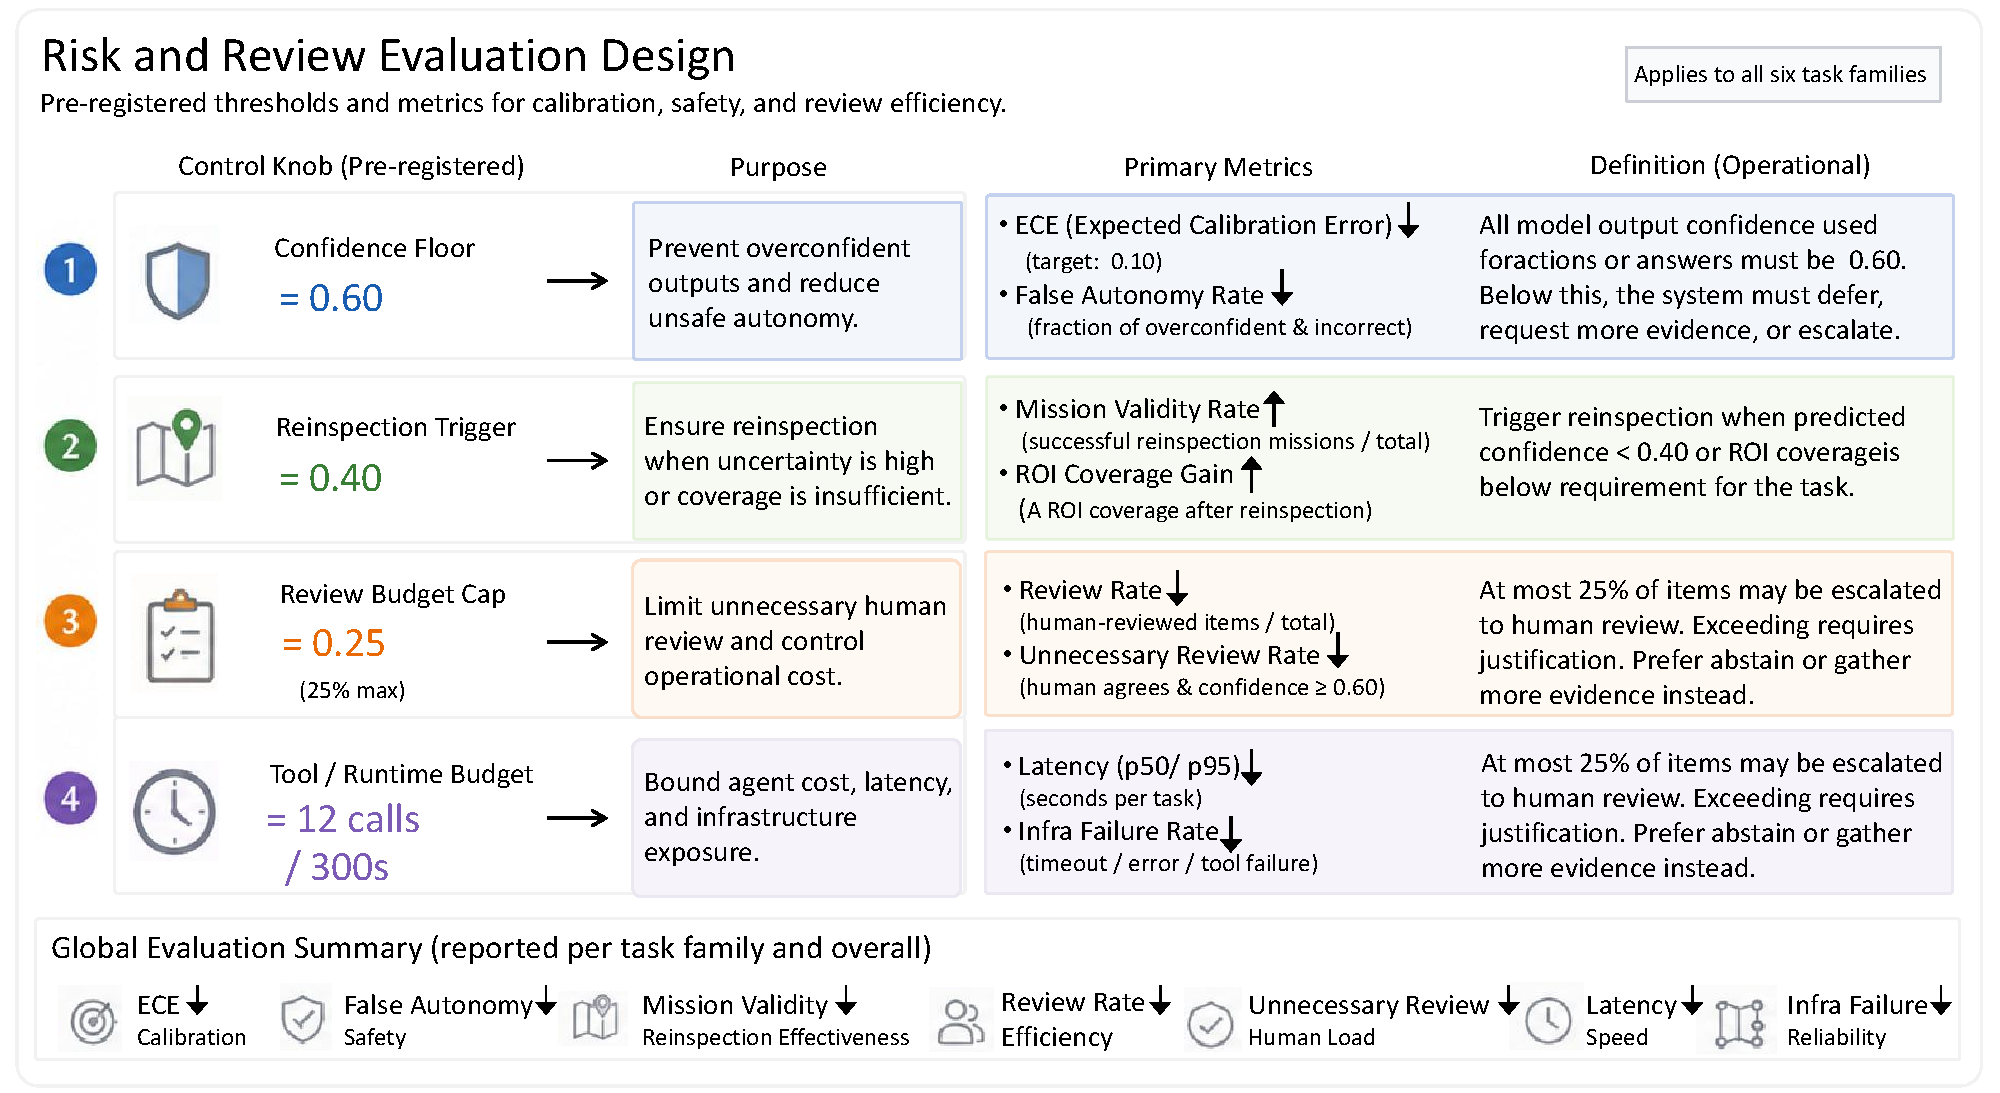
\includegraphics[width=\linewidth]{figs/003}
    \caption{Frozen risk and review quantities used by the formal evaluation protocol. The panel functions as a threshold register for supplementary review analysis rather than as a post-hoc fitted curve.}
    \label{fig:risk-coverage}
\end{figure}

\begin{table}[ht]
    \centering
    \small
    \setlength{\tabcolsep}{4pt}
    \caption{Supplementary robustness and orchestration results. Held-out rows use the materialized supplementary transfer manifests; Full DA in these rows uses the fast bounded evaluation adapter after the non-fast bounded path timed out on the hazard slice.}
    \label{tab:orchestration-comparison}
    \begin{tabular}{L{0.22\linewidth}C{0.12\linewidth}C{0.12\linewidth}C{0.12\linewidth}L{0.24\linewidth}}
        \toprule
        Evaluation slice & SA full tools & Full DA & Infra fail & Status \\
        \midrule
        Hazard-held-out & 0.690 & 0.690 & 0.000 & completed on 29-task Earthquake slice \\
        Region-held-out & 0.714 & 0.714 & 0.000 & completed on 77-task Asia-Pacific slice \\
        Time-held-out & 0.779 & 0.779 & 0.000 & completed on 77-task post-2023 slice \\
        Long-horizon & 0.492 & 0.362 & 0.000 & completed formal slice on 130 drone/assessment/report tasks \\
        \bottomrule
    \end{tabular}
\end{table}

\begin{table}[ht]
    \centering
    \small
    \setlength{\tabcolsep}{4pt}
    \caption{Supplementary drone and review results under the same hidden-test execution boundary as the main table. Oracle and main-system reference rows are populated from the frozen runs together with completed review and drone ablations.}
    \label{tab:drone-review}
    \begin{tabular}{L{0.22\linewidth}C{0.10\linewidth}C{0.10\linewidth}C{0.10\linewidth}C{0.10\linewidth}C{0.10\linewidth}C{0.10\linewidth}}
        \toprule
        Variant & Mission & ROI & Assess. & ECE & Review & E2E \\
        \midrule
        Oracle all gold & 1.000 & 1.000 & 1.000 & 0.010 & 0.000 & 1.000 \\
        Oracle grounding single-agent & 0.000 & 1.000 & 1.000 & 0.050 & 0.000 & 0.672 \\
        Full DisasterAgent & 1.000 & 1.000 & 0.114 & 0.686 & 0.000 & 0.683 \\
        w/o Drone Agent & 0.000 & 1.000 & 0.500 & 0.195 & 0.786 & 0.588 \\
        w/o Review Policy & 1.000 & 1.000 & 0.500 & 0.179 & 0.000 & 0.748 \\
        w/o Drone + Review & 0.000 & 1.000 & 0.500 & 0.097 & 0.000 & 0.588 \\
        \bottomrule
    \end{tabular}
\end{table}

\begin{table}[ht]
    \centering
    \small
    \setlength{\tabcolsep}{4pt}
    \caption{Supplementary ablation results under the same hidden-test execution boundary as the main table. Rows report completed component removals and the matched single-agent replacement baseline.}
    \label{tab:ablation}
    \begin{tabular}{L{0.24\linewidth}C{0.10\linewidth}C{0.10\linewidth}C{0.10\linewidth}L{0.34\linewidth}}
        \toprule
        Variant & E2E & Assess. & Report & Interpretation \\
        \midrule
        Oracle all gold & 1.000 & 1.000 & 1.000 & oracle ceiling under the frozen scorer \\
        Oracle grounding single-agent & 0.672 & 1.000 & 0.278 & removes assessment ambiguity but not drone/report bottlenecks \\
        Full DisasterAgent & 0.683 & 0.114 & 0.222 & multi-agent reference \\
        w/o Data Agent & 0.733 & 0.500 & 0.278 & removes retrieval-specialized delegation while preserving downstream structure \\
        w/o Model Agent & 0.752 & 0.523 & 0.222 & removes model-side perception support; report grounding remains the main loss \\
        w/o Drone Agent & 0.588 & 0.500 & 0.278 & collapses the drone family and lowers end-to-end completion \\
        w/o Review Loop & 0.748 & 0.500 & 0.278 & preserves task score but suppresses review-triggered governance \\
        w/o Workflow Bridge & 0.748 & 0.500 & 0.278 & preserves task score while increasing review activity and tool overhead \\
        w/o HEG & 0.748 & 0.500 & 0.278 & preserves task score while increasing tool calls and review pressure \\
        Single-agent replacement & 0.748 & 0.500 & 0.278 & populated by the formal single-agent full-tools run \\
        \bottomrule
    \end{tabular}
\end{table}

\section{Trace-Grounded Prototype Diagnostics}

We classify failures into wrong event retrieval, wrong map-source grounding, localization miss, wrong reinspection mode or route, temporal mismatch, conflicting evidence, and overconfident report generation. Figure~\ref{fig:case-study} instantiates this diagnostic view using representative traces selected to complement the formal hidden-test summary with trace-level attribution.

\begin{figure}[ht]
    \centering
    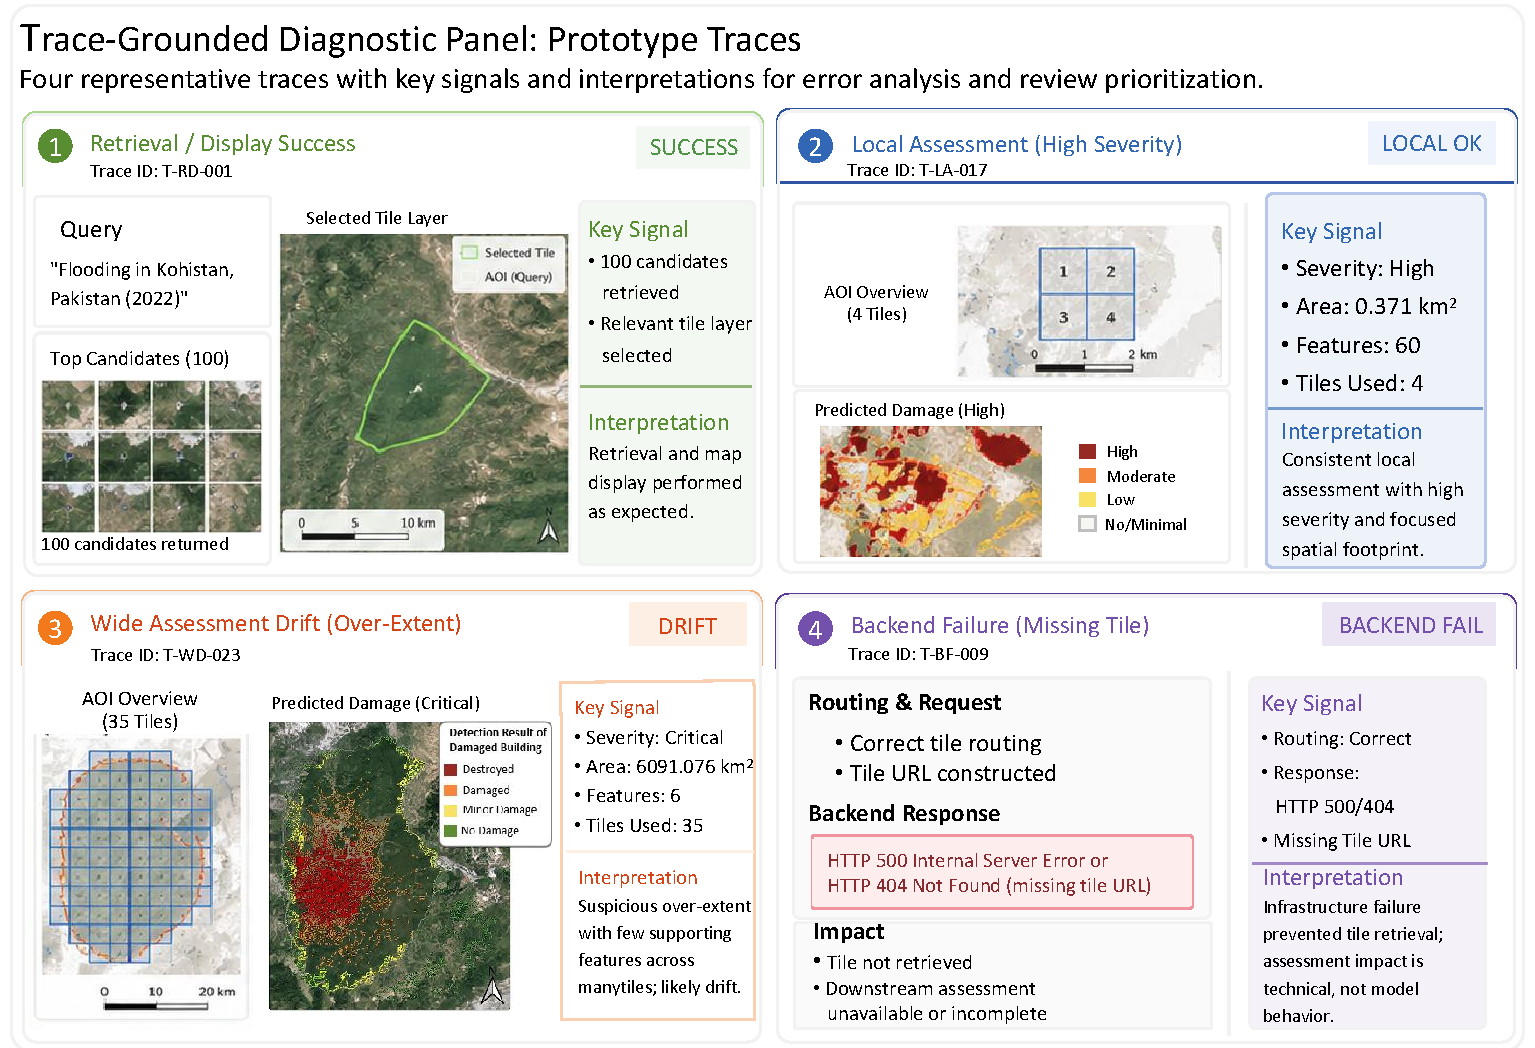
\includegraphics[width=\linewidth]{figs/004}
    \caption{Trace-grounded diagnostic panel built from one retrieval-display trace, two completed assessment traces, and one model-detect failure. The table emphasizes measurable signals and failure attribution rather than a narrative workflow diagram.}
    \label{fig:case-study}
\end{figure}

\section{Supplementary Benchmark Context}

This appendix records supplementary benchmark context, including split metadata, family composition, frozen policy files, and reproducibility-oriented run structure. These details are included to support inspection without interrupting the main-paper narrative.

\section{Split Manifest Summary}
\label{sec:split-manifest-summary}

\begin{table}[ht]
    \centering
    \small
    \caption{Split and hidden-test composition over hazard-event units. The counts are computed from the split manifest metadata; the final row records the hidden-test task set used for the evaluation tables.}
    \label{tab:split-summary}
    \begin{tabular}{lccccc}
        \toprule
        Split & Units & Hazards & Paired & Area-only & Label-only \\
        \midrule
        Train & 212 & 20 & 29 & 182 & 1 \\
        Dev & 46 & 15 & 2 & 42 & 2 \\
        Hidden test & 46 & 15 & 5 & 39 & 2 \\
        Hidden-test tasks & 262 & 6 fam. & -- & -- & -- \\
        \bottomrule
    \end{tabular}
\end{table}

The split manifest preserves broad hazard coverage while still reflecting the underlying supervision asymmetry of the source bundle. Across all 304 units, the largest hazard families are flooding (65), Hurricane (49), and Earthquake (33). The hidden-test split remains intentionally diverse despite its small size, with its largest families being flooding (10), Hurricane (7), and Earthquake (5), followed by several hazards with one to three events each. This is sufficient for a first benchmark version, but the paper should still report per-family task counts after task instantiation is fixed.

\section{Task-Family Composition and Eligibility Policy}

\begin{table}[ht]
    \centering
    \small
    \caption{Task-family eligibility and hidden-test counts. The table records how each family is instantiated from the split manifest and frozen supervision artifacts.}
    \label{tab:family-eligibility}
    \begin{tabular}{L{0.19\linewidth}L{0.29\linewidth}L{0.17\linewidth}L{0.23\linewidth}}
        \toprule
        Family & Minimum manifest-side requirement & Current hidden-test count & Primary frozen supervision \\
        \midrule
        Event retrieval & Hazard-event unit assigned to a split & 44 hidden-test tasks & canonical event identifier \\
        Map grounding & Retrieval-eligible unit plus canonical displayable source or layer & 44 hidden-test tasks & display source or layer target \\
        Damage localization & \texttt{has\_area} or \texttt{has\_label} & 44 hidden-test tasks & geometry target and threshold rule \\
        Drone reinspection & \texttt{has\_area} for ROI construction & 42 hidden-test tasks & mission template and interrupt policy \\
        Assessment synthesis & Localization-eligible unit plus severity target and evidence keys & 44 hidden-test tasks & severity target plus evidence keys \\
        Report generation & Assessment-eligible unit plus output schema & 44 hidden-test tasks & report slot contract and grounding rule \\
        \bottomrule
    \end{tabular}
\end{table}

This table makes explicit which supervision file anchors each task family. It is useful for understanding why the benchmark separates geometry-centric performance from assessment/report performance and why the latter families depend on additional evidence and slot-level constraints.

\section{Execution Artifacts}

The repository includes several benchmark assets that are useful for converting the draft into a fully evaluated submission:
\begin{itemize}[leftmargin=1.2em]
    \item a split-manifest file with 212 train units, 46 development units, and 46 hidden-test units;
    \item workflow-trace summaries covering completed display, assessment, and mixed retrieval-assessment executions together with a small number of failed detection traces;
    \item assessment summaries confirming that the pipeline emits disaster-type and severity labels before formal scoring;
    \item a repository-local freeze package containing the severity glossary, impact-fact format, evidence-key registry, report template, and package manifest;
    \item a hidden-test package containing the frozen evaluation configuration, hidden-test manifest metadata, and 262 gold-removed task records.
\end{itemize}

These files should not be interpreted as formal system-performance results. Instead, they serve as benchmark assets, qualitative case-study evidence, and sanity checks on the execution pipeline.

\section{Severity and Evidence Freeze Protocol}

Assessment and report tasks are structurally present in the hidden-test package, with 44 task records per family. Assessment summaries also confirm that the pipeline emits disaster type and severity labels before formal scoring, with observed labels spanning multiple disaster types and severity levels. These summaries are diagnostic artifacts rather than benchmark gold. The repository includes a frozen core-policy package together with adjudication-ready task-level assessment and report overrides, which make the final hidden-test evaluation possible.

\begin{table}[ht]
    \centering
    \small
    \setlength{\tabcolsep}{3pt}
    \caption{Current freeze-package status. Core policy files are frozen, and task-level hidden-test assessment/report overrides are maintained as adjudication-controlled benchmark artifacts.}
    \label{tab:severity-freeze}
    \begin{tabular}{L{0.22\linewidth}L{0.19\linewidth}L{0.31\linewidth}L{0.18\linewidth}}
        \toprule
        Artifact & Schema fields & Freeze rule & Current workspace signal \\
        \midrule
        Severity label glossary & \texttt{severity} & Lock label names and ordinals before distribution & 5 labels frozen: none--critical \\
        Impact fact format & \texttt{impact facts} & Store atomic, source-grounded facts only & Core format frozen \\
        Evidence-key registry & \texttt{evidence keys} & Freeze a controlled key vocabulary and source types & 11 evidence keys frozen \\
        Report template & \texttt{report slots + metrics} & Freeze required slots and evidence-coverage rule & 5 slots; grounding threshold 0.8 \\
        Assessment overrides & \texttt{severity + facts} & Live file should contain adjudicated rows only & 44 hidden-test rows prepared for formal use \\
        Report overrides & \texttt{facts + slots} & Live file should contain adjudicated rows only & 44 hidden-test rows prepared for formal use \\
        \bottomrule
    \end{tabular}
\end{table}

With adjudicated override rows in place, assessment and report tasks can be scored under the same formal hidden-test protocol as the rest of the benchmark. The remaining challenge is therefore no longer benchmark design, but improving semantic assessment and report quality under the frozen protocol.

\section{Reproducibility Protocol}
\label{sec:execution-plan}

This section records the reproducibility protocol used to bind each reported number to a fixed split, a fixed task subset, a saved prediction file, and a pre-declared statistical rule.

\paragraph{Stage 0: Freeze benchmark artifacts.}
Before any model comparison, freeze four benchmark files: (1) the event-level split manifest; (2) the finalized task records with task family, difficulty, and gold fields; (3) a hidden-test package with gold outputs removed; and (4) an evaluation configuration file containing metric thresholds, review thresholds, and the seed list. For assessment and report tasks, this freeze also includes the severity/evidence package described in Table~\ref{tab:severity-freeze}: the severity label glossary, impact-fact format, evidence-key registry, and report template. In the repository these core files are already frozen, and adjudicated hidden-test overrides are maintained under the same controlled boundary. No prompts, routing rules, threshold values, or grading thresholds may change after this freeze point.

\paragraph{Stage 1: Validate the benchmark itself.}
Run benchmark-quality checks before system evaluation. Specifically, report split coverage by hazard and supervision type, dual-annotation agreement on a stratified subset, oracle execution validity for each task family, and human-reference solvability on a small but difficulty-balanced subset. If a task family fails these checks, revise the benchmark before populating any system-comparison table.

\paragraph{Stage 2: Tune once on development data.}
Use only the public Event-IID development split for prompt editing, workflow routing, review-threshold selection, and detector-mode selection. Thresholds for review and reinspection should be selected to optimize a declared development objective such as severity F1 at a false-autonomy cap or end-to-end score under a review-budget cap. After tuning, freeze one configuration per system and reuse it unchanged for hidden-test and transfer evaluation.

\paragraph{Stage 3: Run the main Event-IID evaluation.}
Evaluate the comparison systems on the Event-IID hidden-test split summarized in Table~\ref{tab:main-results}. Deterministic systems may be run once; stochastic systems should be run with three seeds using the same task order and tool budget. Save one prediction file and one execution trace bundle per seed. The hidden-test scorer should emit per-task metrics, family-level aggregates, end-to-end success, latency, tool calls, and a failure tag in \{\texttt{success}, \texttt{reasoning\_failure}, \texttt{infra\_failure}, \texttt{policy\_review}\}.

\paragraph{Stage 4: Run transfer and orchestration robustness.}
Populate Table~\ref{tab:orchestration-comparison} using the same frozen system configurations. Evaluate the selected systems on hazard-held-out, region-held-out, and time-held-out splits, then run a separate long-horizon subset containing tasks that require at least three state-bearing stages such as retrieval$\rightarrow$grounding$\rightarrow$assessment or retrieval$\rightarrow$localization$\rightarrow$drone. Report infrastructure-failure rate separately rather than folding it into task error.

\paragraph{Stage 5: Run drone and review variants.}
Populate Table~\ref{tab:drone-review} on the subset of hidden-test tasks that are drone-eligible or review-eligible. Compare the full system against variants without the Drone Agent, without review routing, and without both. Mission validity and ROI coverage should be averaged only over tasks with a gold drone target; severity F1, ECE, review rate, and false-autonomy rate should be computed over the full eligible subset.

\paragraph{Stage 6: Run ablations.}
Table~\ref{tab:ablation} should use the Event-IID hidden-test split with the same frozen prompts and thresholds as the main system. The purpose of this table is not to retune every ablation independently, but to measure what breaks when key components are removed. This keeps the comparison operationally honest.

\paragraph{Per-table filling rules.}
The paper can now be populated mechanically:
\begin{itemize}[leftmargin=1.2em]
    \item \textbf{Table~\ref{tab:main-results}.} Use Event-IID hidden-test only; columns Retr., Ground., Local., Drone, Assess., and Report should be family-level primary metrics, and E2E should be the percentage of tasks whose primary criterion is met end to end.
    \item \textbf{Table~\ref{tab:orchestration-comparison}.} Use hazard-held-out, region-held-out, time-held-out, and long-horizon subsets only. Do not mix Event-IID numbers into this table.
    \item \textbf{Table~\ref{tab:drone-review}.} Restrict mission validity and ROI coverage to drone-eligible tasks. Severity F1, ECE, review rate, FAR, and E2E should use the full review/drone-eligible subset with frozen thresholds.
    \item \textbf{Table~\ref{tab:ablation}.} Use the same Event-IID hidden-test tasks as the main system row so that deltas remain interpretable.
\end{itemize}

\paragraph{Metric-to-family mapping.}
Each task family should have one declared primary score used in the family column of Table~\ref{tab:main-results}: event retrieval uses top-1 event accuracy; map grounding uses grounding success against the correct source or layer; damage localization uses GeoJSON F1 or IoU with thresholded partial credit; drone reinspection uses mission validity as the primary score and ROI coverage as an auxiliary score; assessment synthesis uses severity F1; and report generation uses report grounding score against required evidence keys. End-to-end success is defined per task record by its primary metric and threshold.

\paragraph{Required run artifacts.}
Each evaluated run should save the following files in a stable directory structure:
\begin{enumerate}[leftmargin=1.2em]
    \item \texttt{config.json}: frozen prompt revision, tool budget, threshold values, and seed;
    \item \texttt{predictions.jsonl}: one record per task with raw outputs and normalized predictions;
    \item \texttt{trace.jsonl}: ordered tool calls, intermediate states, and timestamps;
    \item \texttt{metrics.json}: aggregate metrics, calibration summaries, and failure counts;
    \item \texttt{failures.csv}: task ID, failure type, and a short diagnostic note.
\end{enumerate}

\paragraph{Stable run-directory convention.}
To keep table generation mechanical rather than notebook-driven, we recommend a fixed directory layout of the form \path{runs/<subset>/<system>/<config_id>/seed_<k>/}. Here \texttt{subset} is one of Event-IID hidden test, hazard-held-out, region-held-out, time-held-out, long-horizon, or drone/review evaluation; \texttt{config\_id} identifies the frozen prompt and threshold package; and each seed directory contains exactly the five files listed above. Human-reference runs may use \texttt{seed\_human} in place of a numeric seed, but should still emit the same file names so that table scripts do not need a separate code path.

\paragraph{Table-to-subset mapping.}
Once this layout is fixed, each table should draw from exactly one family of run directories:
\begin{itemize}[leftmargin=1.2em]
    \item \textbf{Table~\ref{tab:main-results}} reads only Event-IID hidden-test runs.
    \item \textbf{Table~\ref{tab:orchestration-comparison}} reads only hazard-held-out, region-held-out, time-held-out, and long-horizon runs.
    \item \textbf{Table~\ref{tab:drone-review}} reads only drone/review runs.
    \item \textbf{Table~\ref{tab:ablation}} reads only Event-IID hidden-test ablation runs produced under the same \texttt{config\_id} as the full system.
\end{itemize}

\paragraph{Statistical reporting.}
For stochastic systems, compute the main score for each seed, pool task-level predictions across seeds only where the metric definition permits it, and report means with 95\% bootstrap confidence intervals. Pairwise claims against the full DisasterAgent row should use paired bootstrap or approximate randomization over the same hidden-test tasks. The paper should avoid significance testing on development data because that split is used for tuning.

\paragraph{Interpreting repeated seeds.}
Several supplementary systems in the evaluation stack are near-deterministic under the frozen benchmark boundary. In particular, the heuristic single-agent and ablation baselines often differ across seeds only in continuous auxiliary quantities such as latency or calibration, while thresholded family metrics and end-to-end success remain identical. The full-DisasterAgent configuration is also relatively stable because routing, thresholds, and task order are locked and several expensive background branches are disabled for reproducible formal execution. Accordingly, repeated seeds in this study should be read primarily as a stability check on the frozen evaluation path rather than as an attempt to estimate large stochastic variance.

\paragraph{Artifact status.}
The repository contains a split manifest over 212/46/46 train/dev/hidden-test hazard-event units, a task schema with family and metric fields, trace summaries that expose both successful assessments and infrastructure failures, a frozen core-policy package, a hidden-test task package, and formal hidden-test run artifacts for the completed main-table systems. The package includes a frozen evaluation configuration, hidden-test manifest metadata, and 262 gold-removed task records. The freeze package includes severity labels, impact-fact schema, evidence-key registry, report-slot contract, and controlled task-level assessment/report overrides.

\paragraph{Supplementary experiment status.}
The main hidden-test comparison in Table~\ref{tab:main-results} is complete under the frozen evaluation boundary, and the appendix now also includes populated long-horizon, drone/review, ablation, validation, and materialized held-out transfer diagnostics. The remaining caveat is therefore no longer missing rows, but \emph{execution-mode comparability}: the held-out transfer rows use the fast bounded evaluation adapter for Full DisasterAgent after the non-fast bounded path timed out on the first hazard slice attempt. If later revisions replace those rows, they should do so under the same frozen scorer, manifests, and file contract so that the updated transfer numbers remain directly comparable to the current appendix tables.

\section{Task Record Summary}

The task schema stores:
\begin{itemize}[leftmargin=1.2em]
    \item task metadata: task ID, split, family, difficulty;
    \item execution constraints: allowed tools and tool budget;
    \item context: candidate events, pre/post assets, seed map source, region of interest, simulator start state;
    \item gold outputs: event ID, hazard type, map source, target region or GeoJSON, drone mission targets, allowed interrupts, minimum coverage, severity, evidence keys;
    \item evaluation settings: primary metric, auxiliary metrics, grading thresholds;
    \item provenance: event name, hazard type, region, source bundle, review requirement, operator-control level, annotation status.
\end{itemize}

\section{Artifact Summary}

The package stack supporting this paper has three layers:
\begin{enumerate}[leftmargin=1.2em]
    \item benchmark-definition artifacts: split metadata, task schema, hidden-test task package, and frozen evaluation configuration;
    \item policy artifacts: severity labels, evidence-key registry, impact-fact schema, report template, and task-level overrides;
    \item execution artifacts: prediction files, trace bundles, aggregate metrics, and failure summaries for formal runs.
\end{enumerate}

\end{document}
